\documentclass{beamer}
\usetheme{Warsaw}

\usepackage[utf8]{inputenc}
\usepackage{fancybox}
\usepackage{multimedia} 
\usepackage{subfig}
\usepackage{amsmath}
\usepackage{hyperref}
\usepackage[all]{xy}
\usepackage{algorithm}
%\usepackage{arevmath}     % For math symbols
\usepackage[noend]{algpseudocode}
\setbeamertemplate{footline}[frame number]

% Define custom commands for \EE, \Tau, and \MM
\newcommand{\EE}{\mathcal{E}}
\newcommand{\Tau}{\mathcal{T}}
\newcommand{\MM}{\mathcal{M}}
\renewcommand{\Pr}{\mathbb{P}}

\begin{document}



\title[Stochastik] % (optional, only for long titles)
{Stochastik für Informatiker
\\
\includegraphics[scale=0.5]{img/craps}
}
\subtitle{}
\author[Dr. Johannes Riesterer] % (optional, for multiple authors)
{Dr.  rer. nat. Johannes Riesterer}

\date[KPT 2004] % (optional)
{}

\subject{Stochastik}

\begin{frame}
    \frametitle{Motivation}
\framesubtitle{}
\begin{figure}[htp]
      \centering
    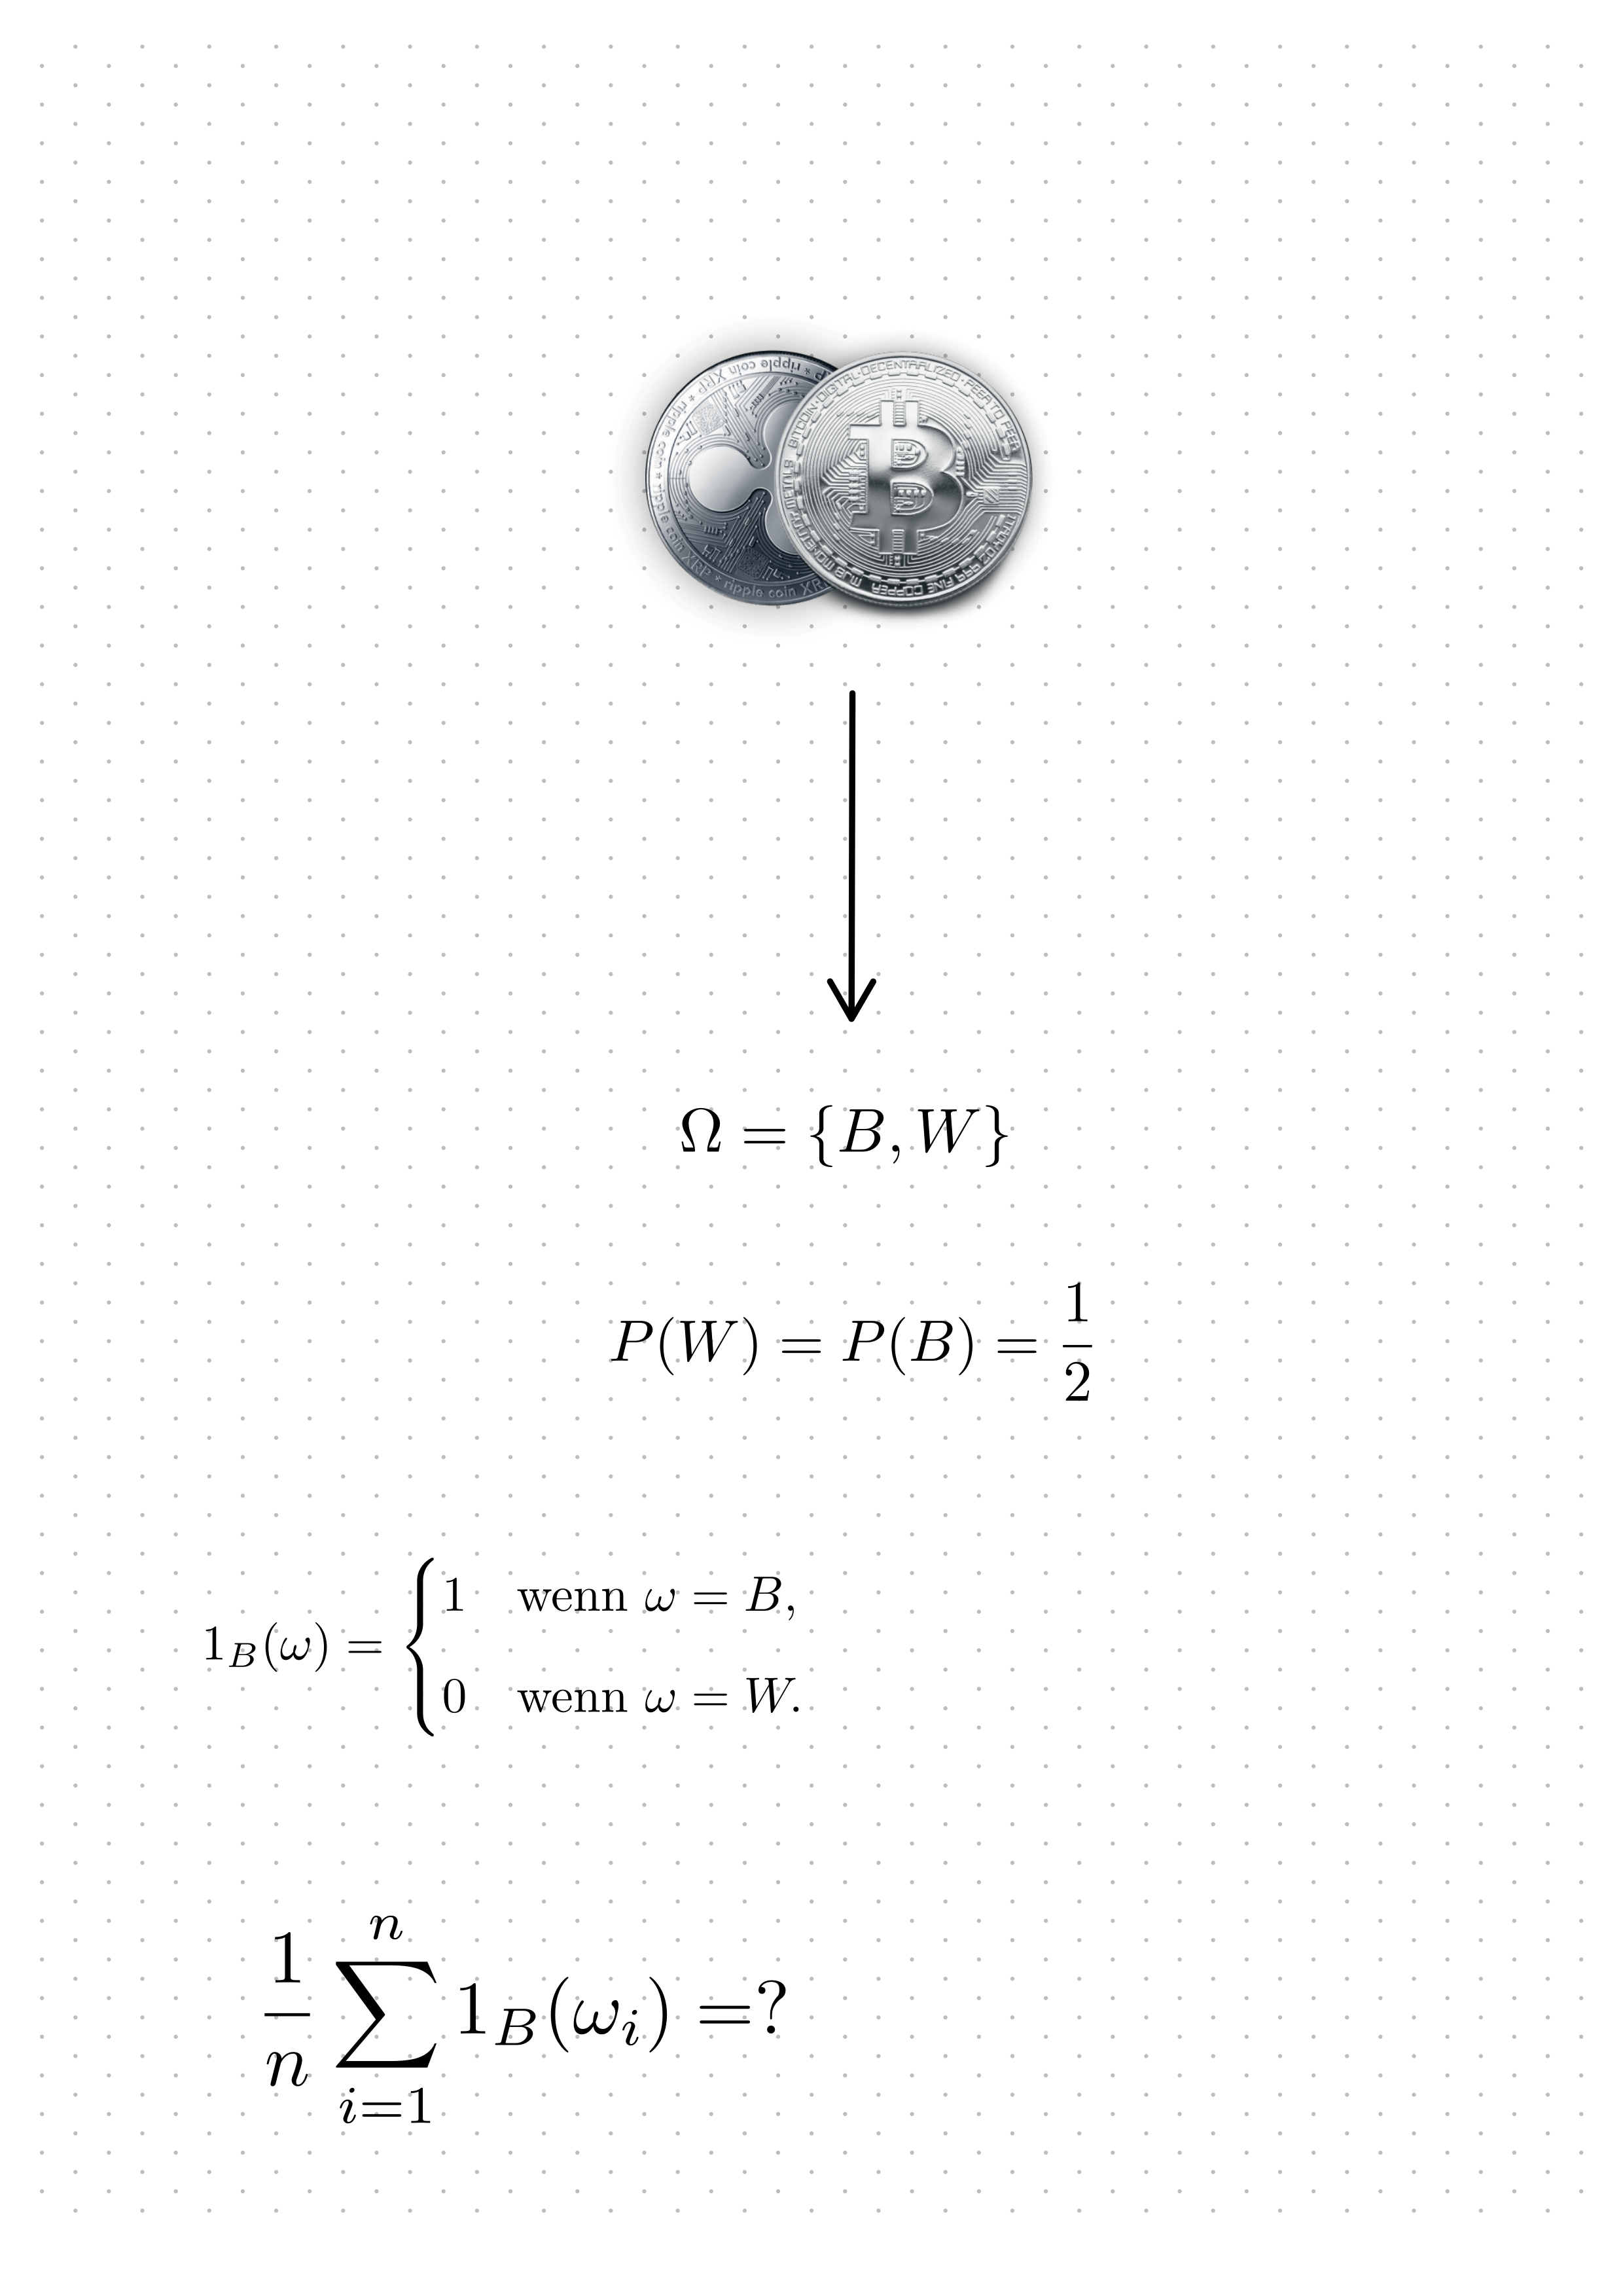
\includegraphics[width=0.6\textwidth]{img/coinflip.png}
\end{figure}
 \end{frame}


 \begin{frame}
    \frametitle{Integration}
\framesubtitle{}
Archimedes von Syrakus  um 287 v. Chr. vermutlich in Syrakus; † 212 v. Chr. ebenda) war ein griechischer Mathematiker, Physiker und Ingenieur. Er gilt als einer der bedeutendsten Mathematiker der Antike. Seine Werke waren auch noch im 16. und 17. Jahrhundert bei der Entwicklung der höheren Analysis von Bedeutung. 

\begin{figure}[htp]
      \centering
    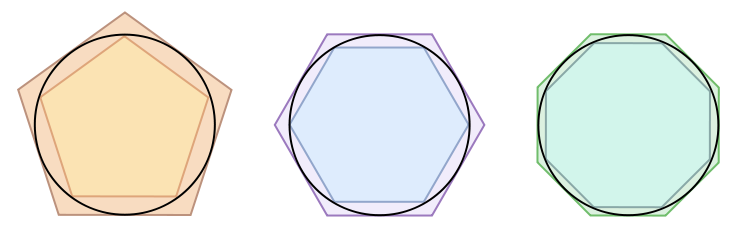
\includegraphics[width=0.6\textwidth]{img/750px-Archimedes_pi.png}
\end{figure}
 \end{frame}



\begin{frame}
    \frametitle{Stochastik}
\framesubtitle{Inegrierbare Funktionen}
    \begin{block}{Maßraum}
     Ein Meßraum $(\Omega, \mathcal{A})$ ist ein Tupel bestehend aus der Grundmenge $\Omega$ und einer $\sigma$-Algebra $\mathcal{A} \subset  \mathcal{P}(\Omega)$ 
\end{block}

\begin{block}{Maß}
    Ein Maß auf einem Meßraum $(\Omega, \mathcal{A})$ ist Abbildung
    $\mu : \mathcal{A} \to \mathbb{R}_{\geq 0}$
    \begin{align*}
    \mu \biggl(  \bigcup_i A_i  \biggr) = \sum_i \mu(A_i), \text{ mit } A_i \cap A_j = \emptyset \text{ für } i \neq j
    \end{align*}
    \end{block}
    
    \begin{block}{Wahrscheinlichkeitsmaß}
     Ein Maß mit $\mu (\Omega) = 1$ ist ein Wahrscheinlichkeitsmaß.
   \end{block}

 \end{frame}


  
 \begin{frame}{Stochastik}
    \framesubtitle{Sigma-Algebra}
    \begin{block}{erzeugte Sigma-Algebra}
    Sei $X$ eine Menge und $\mathcal{C}\subseteq\mathcal{P}(X)$ ein Mengensystem.\\[0.5em]
    Die von $\mathcal{C}$ erzeugte $\sigma$‑Algebra ist definiert als
    \[
      \sigma(\mathcal{C})
      =
      \bigcap\bigl\{\mathcal{F}\subseteq\mathcal{P}(X)\;\bigm|\;
        \mathcal{F}\text{ ist eine $\sigma$‑Algebra und }\mathcal{C}\subseteq\mathcal{F}\bigr\}.
    \]
    \end{block}
  \end{frame}
  
  \begin{frame}{Stochastik}
    \framesubtitle{Sigma-Algebra}
    \begin{itemize}
      \item $\mathcal{P}(X)$ selbst ist eine $\sigma$‑Algebra und enthält $\mathcal{C}$.  
      \item Daher ist die Menge aller $\sigma$‑Algebren, die $\mathcal{C}$ enthalten, nicht leer.  
      \item Der Schnitt beliebig vieler $\sigma$‑Algebren ist wieder eine $\sigma$‑Algebra.  
      \item Damit existiert und ist eindeutig die kleinste $\sigma$‑Algebra mit $\mathcal{C}\subseteq\sigma(\mathcal{C})$.

      \item $\sigma(\mathcal{C})$ enthält genau diejenigen Mengen, die aus $\mathcal{C}$ gewonnen werden können durch
      
          \item Komplementbildung,
          \item abzählbare Vereinigungen,
          \item (und folglich abzählbare Durchschnitte).
       \end{itemize}
  \end{frame}
  
  \begin{frame}{}
    \frametitle{Stochastik}
    \framesubtitle{Sigma-Algebra}
\begin{block}{Borellsche Sigma-Algebra auf $\mathbb{R}$}
    Die \emph{Borel‑$\sigma$‑Algebra} $\mathcal B(\mathbb R)$ ist definiert als
    \[
      \mathcal B(\mathbb R)
      =
      \sigma\bigl(\{\text{offene Teilmengen von }\mathbb R\}\bigr).
    \]
    Äquivalent:
    \begin{align*}
      \mathcal B(\mathbb R)
      &= \sigma\bigl(\{(a,b):a<b\}\bigr)
      = \sigma\bigl(\{(-\infty,a):a\in\mathbb R\}\bigr).
    \end{align*}
\end{block}
  \end{frame}

  

  \begin{frame}{Inklusion 2: offene Intervalle}
    Jede offene Menge $U$ lässt sich darstellen als
    \[
      U=\bigcup_{k=1}^\infty(a_k,b_k),\quad a_k,b_k\in\mathbb Q.
    \]
   
    \[
      (a,b)=(-\infty,b)\cap(( -\infty,a])^c
    \]
    \[
      (-\infty,a]=\bigcap_{n=1}^\infty(-\infty,a+\tfrac1n)\in\sigma(\mathcal H)
    \]
  

    
  \end{frame}

  
 \begin{frame}
    \frametitle{Stochastik}
\framesubtitle{Inegrierbare Funktionen}
    \begin{block}{Meßbare Abbildung}
     Eine Abbildung $f:\Omega \to \Omega'$ zwischen zwei Maßräumen 
      $(\Omega, \mathcal{A})$ und $(\Omega', \mathcal{A}')$ heißt meßbar, falls
    \begin{align*}
        f^{-1}(A') \in \mathcal{A} \; \text{für alle } A' \in \mathcal{A}'
    \end{align*}
    \end{block}

    \begin{block}{Meßbare Abbildung}
    Das Urbild jedes Ereignisses ist ein Ereignis
    \end{block}

    \begin{block}{Beispiel}
        Bei endlichen Mengen mit der Potenzmenge als Sigma-Algebra ist jede Funktion Meßbar.
    \end{block}

    
 \end{frame}


\begin{frame}
    \frametitle{Stochastik}
\framesubtitle{}
    \begin{block}{Meßbare Funktionen }
        Die Menge der meßbaren Funktionen $f: \Omega \to \mathbb{R}$ bezeichnen wir mit $\mathcal{M}_\Omega$ oder einfach $\mathcal{M}$
        wenn der Kontext klar ist. 
        Mit $\mathcal{M}^+$ bezeichnen wir die meßbaren Funktionen $f: \Omega \to \mathbb{R}$ mit $f(\omega) \geq 0$. 
    \end{block}

\end{frame}

\begin{frame}{Satz}
    \frametitle{Stochastik}
    \framesubtitle{}
    \begin{block}{Messbarkeit von Abbildungen}
      Sei $(X,\Sigma)$ ein Messraum, $Y$ eine Menge und
      \[
        \EE \;\subseteq\;\mathcal P(Y),
        \quad
        \Tau = \sigma(\EE)
      \]
      die von $\EE$ erzeugte $\sigma$‑Algebra auf $Y$. Dann ist
      \[
        f\colon (X,\Sigma)\;\longrightarrow\;(Y,\Tau)
      \]
      genau dann messbar, wenn
      \[
        f^{-1}(E)\in\Sigma
        \quad\text{für alle }E\in\EE.
      \]
    \end{block}
  \end{frame}
  



\begin{frame}
    \frametitle{Stochastik}
\framesubtitle{}
\begin{block}{Indikatorfunktion}
    Für eine Teilmenge $A \subset \Omega$ heißt
    $$ 1_A (x): = \begin{cases} 1 \text{  falls }   x \in A  \\  0  \text{  sonst}  \end{cases}$$
    Indikatorfunktion.
    \end{block}
    
    \begin{figure}[H]
          \centering
        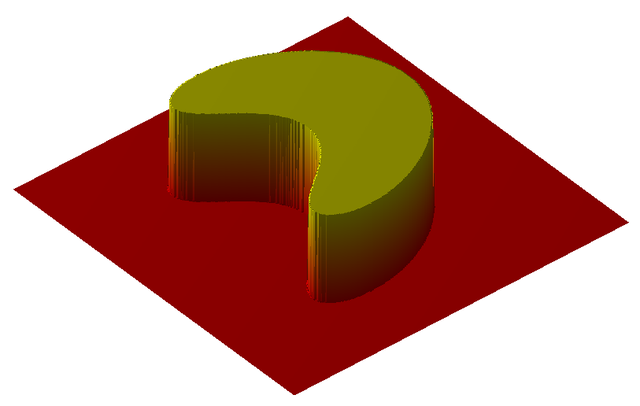
\includegraphics[width=0.5\textwidth]{img/640px-Indicator_function_illustration}
          \caption{Quelle: Wikipedia: https://commons.wikimedia.org/wiki/File:Indicator\_function\_illustration.png}
    
    \end{figure}
\end{frame}



\begin{frame}
    \frametitle{Stochastik}
\framesubtitle{}
    \begin{block}{Treppenfunktion}
        Eine meßbare Funktion $u: \Omega \to \mathbb{R}$ 
        heißt Treppenfunktion, 
        falls sie nur endlich viele verschiedene Werte annimmt.
    \end{block}


\begin{figure}[H]
    \centering
  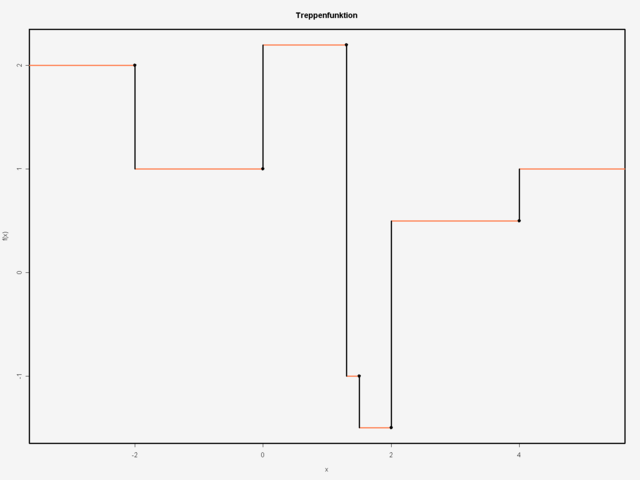
\includegraphics[width=0.6\textwidth]{img/640px-Stepfunction1}
    \caption{Quelle: Wikipedia: https://commons.wikimedia.org/wiki/File:Stepfunction1.png}

\end{figure}
\end{frame}



\begin{frame}
    \frametitle{Stochastik}
\framesubtitle{}

    \begin{block}{Beispiel  einer Treppenfuntkion}
         $u(x) = \sum_{i= 1}^n a_i \cdot  1_{A_i}(x)$ mit $A_i \cap A_j = \emptyset$ für $i \neq j$ ist eine Treppenfunktion.
    \end{block}


    \begin{block}{Treppenfuntkion}
        Eine Treppenfunktion  $u$ hat eine Darstellung
        $u(x) = \sum_{i= 1}^n a_i \cdot  1_{A_i}(x)$ mit $A_i \cap A_j = \emptyset$ für $i \neq j$ ist eine Treppenfunktion.
   \end{block}


    \begin{block}{Treppenfuntkion}
        Die Menge der Treppenfunktionen bezeichnen wir mit $\mathcal{T}$ und die Treppenfunktionen mit $a_i > 0$ mit $\mathcal{T}^+$.        
    \end{block}
    


\end{frame}


\begin{frame}
    \frametitle{Stochastik}
\framesubtitle{}

    \begin{block}{Eindeutigkeit der Darstellung}
        Sind $u = \sum_{i= 1}^n a_i 1_{A_i} = \sum_{j= 1}^m b_j 1_{B_j}$ zwei verschiedene Darstellungen einer Treppenfunktion 
        $u \in \mathcal{T}^+$
        so ist $\sum_{i= 1}^n a_i \mu (A_i) = \sum_{j= 1}^m b_j \mu (B_j)$
    \end{block}
    \begin{block}{Beweis}
        \begin{align*}
         u =& \sum_{i= 1}^n a_i \mu (A_i) = \sum_{i= 1}^n \sum_{j= 1}^m a_i \mu (A_i \cap B_j) 
        \\ = & \sum_{i= 1}^n \sum_{j= 1}^m b_j \mu (A_i \cap B_j) = \sum_{j= 1}^m b_j \mu (B_j)       
    \end{align*}
       
    \end{block}    
\end{frame}



\begin{frame}
    \frametitle{Stochastik}
\framesubtitle{}
    \begin{block}{Integral einer Treppenfunktion}
        Für eine Treppenfunktion $u \in \mathcal{T}^+$ definieren wir
\begin{align*}
    \int_\Omega u \; d\mu= \sum_{i=1}^n a_i \mu(A_i)
\end{align*}
Diese ist unabhängig von der Darstellung.
    \end{block}

\end{frame}


\begin{frame}
    \frametitle{Stochastik}
\framesubtitle{}
\begin{block}{Eigenschaften des Integrals von Treppenfunktionen}
    Sind $u$ und $v$ zwei Treppenfunktionen, dann gilt:
    \begin{itemize}
    \item $\int_{\Omega} 1_A  d\mu  = \mu (A)$  
    \item $\int_{\Omega} \alpha u  + \beta v d\mu = \alpha \int_{\Omega}  u d\mu + \beta  \int_{\Omega}  v d\mu$
    \item Ist $u(x) \leq v(x)$ für alle $x$, so ist $\int_{\Omega} u d\mu \leq \int_{\Omega} v d\mu$ 
    \end{itemize}
    \end{block}
\end{frame}



\begin{frame}
    \frametitle{Stochastik}
\framesubtitle{}
    \begin{block}{Integral nicht negativer meßbarer Funktionen}
        Für eine Funktion $f \in \mathcal{M}^+$ definieren wir
        \begin{align*}
            \int_{\Omega} f \;  d \mu := sup \biggl \{ \int_{\Omega} u \; d\mu \; | \; u \in \mathcal{T}^+, u(x) \leq f(x) \text{ für alle } x \in \Omega  \biggr  \}   
        \end{align*}
\end{block}
\end{frame}

\begin{frame}
    \frametitle{Stochastik}
\framesubtitle{}
    \begin{block}{Eigenschaften des Integrals nicht negativer meßbarer Funktionen}
        Seien $f,g :\Omega \to \mathbb{R}_{\geq 0}$ meßbar.
        Dann gilt:
        \begin{itemize}
        \item Ist $f \leq g$ punktweise, dann ist $\int_{\Omega} f  d\mu  \leq \int_{\Omega} g  d\mu$
            \item      Ist   $f_n \in \mathcal{T}^+$ eine punktweise konvergente Folge $f_n \uparrow f$, dann konergierten die Integrale 
            $\int_{\Omega} f  d\mu \uparrow  \int_{\Omega} g  d\mu$
    \end{itemize}
        \end{block}
\end{frame}




\begin{frame} 
    \frametitle{Stochastik}
\framesubtitle{}
    \begin{block}{Meßbare Abbildungen}
        Eine nicht negative messbare Funktion $f:\Omega \to \mathbb{R}_{\geq 0}$ ist genau dann meßbar, wenn
        es eine Folge $f_n \in \mathcal{T}^+$ gibt mit $f_n \uparrow f$.
    \end{block}
    \begin{figure}[H]
        \centering
      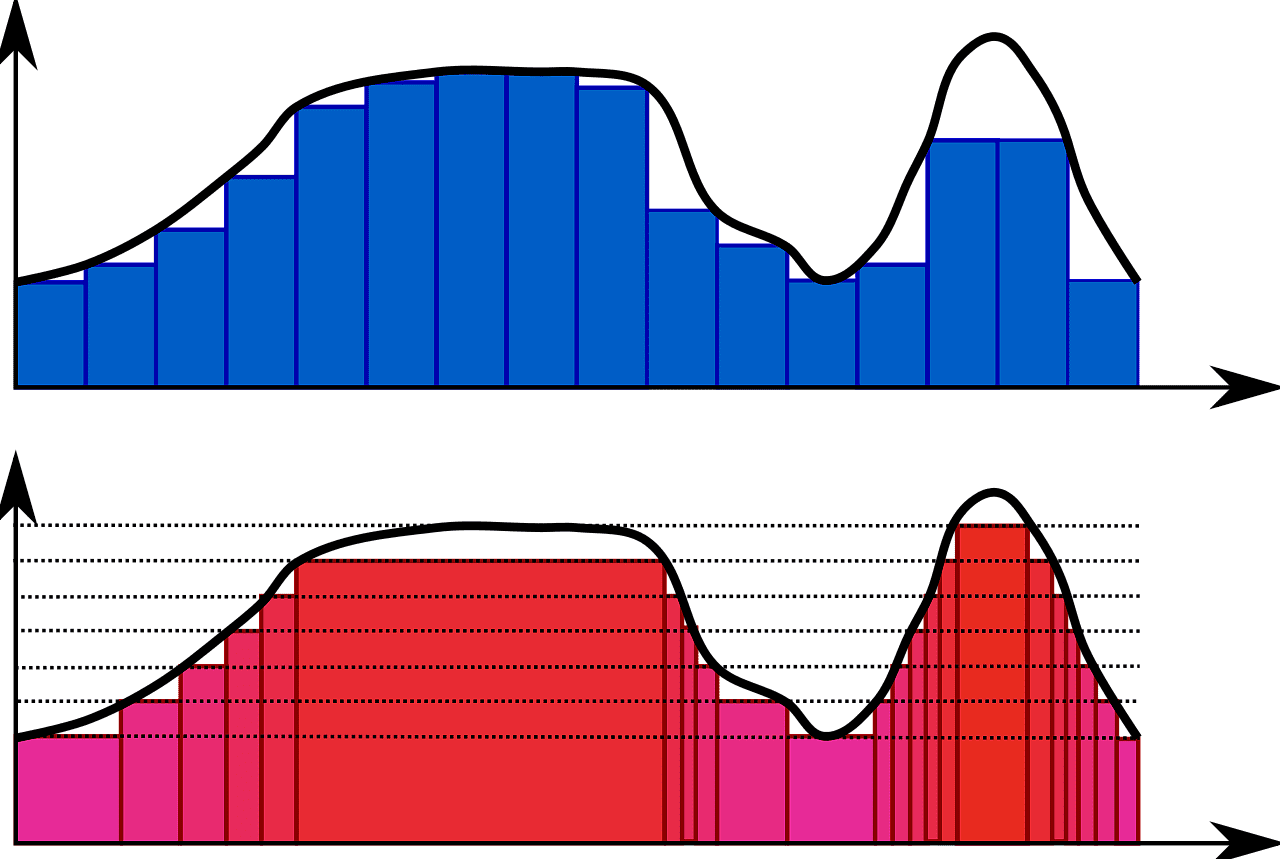
\includegraphics[width=0.6\textwidth]{img/RiemannVsLebesgue.png}
    
    \end{figure}
\end{frame}


\begin{frame}
    \frametitle{Stochastik}
\framesubtitle{}
Sei  $f \in \mathcal{M}^+$ meßbar: \\
definiere
\begin{align*}
    A_{j,n} : = \begin{cases} 
        \{ \frac{j}{2^n} \leq f \leq \frac{j+1}{2^n} \} \text{ für } j= 0, \dots, n \cdot 2^n -1 \\
        \{  f \geq n \} \text{ für } j= n \cdot 2^n 
    \end{cases}
\end{align*}
und damit 
\begin{align*}
    f_n : =  \sum_{j= 0}^{n2^n} \frac{j}{2^n} 1_{A_{j,n}}
\end{align*}
Damit gilt für festes $x$ immer $f_n(x) \leq f(x)$ und man kann $n$ immer so wählen, dass 
$ f(x) \leq f_n(x) +2^{-n}$ gilt.
\end{frame}

\begin{frame}
    \frametitle{Stochastik}
\framesubtitle{}
Sei 
\[
  f_n(x) \;=\; \sum_{i=1}^{k_n} a_{n,i}\,\mathbf{1}_{A_{n,i}}(x),
\]
 eine punktweise konvergente folge $f_n \uparrow f$ von Treppenfunktionen.

\begin{enumerate}
    \item[\textbf{1.}] \emph{Treppenfunktionen sind messbar.} \\
      Für feste $n$ und $\alpha\in\mathbb{R}$ gilt
      \[
        \{x: f_n(x)<\alpha\}
        = \bigcup_{\substack{1\le i\le k_n \\ a_{n,i}<\alpha}} A_{n,i}
        \;\in\;\Sigma,
      \]
      da endliche und abzählbare Vereinigungen sowie Komplemente in $\Sigma$ liegen. Also ist $f_n$ messbar.
  
    \item[\textbf{2.}] \emph{Charakterisierung der Messbarkeit.} \\
      Eine Funktion $g\colon X\to\mathbb{R}$ ist genau dann messbar, wenn für alle $\alpha\in\mathbb{R}$
      \[
        \{x:g(x)<\alpha\}\;\in\;\Sigma.
      \]
  
    
     
    \end{enumerate}
    \end{frame}

    \begin{frame}
        \frametitle{Stochastik}
    \framesubtitle{}
       Da $f_n(x)\to f(x)$ punktweise, gilt für jedes $x\in X$ und jedes $\alpha\in\mathbb{R}$:
      \[
        f(x)<\alpha
        \quad\Longleftrightarrow\quad
        \exists\,k\;\forall\,n\ge k:\;f_n(x)<\alpha.
      \]
    Daher
    \[
      \{x:f(x)<\alpha\}
      = \bigcup_{k=1}^{\infty}\bigcap_{n=k}^{\infty}\{x:f_n(x)<\alpha\}.
    \]

\end{frame}
 



\begin{frame}
    \frametitle{Stochastik}
\framesubtitle{}
    \begin{block}{Integral für meßbare Funktionen}
        Für eine meßbare Funktion  $f \in \mathcal{M}$ setzen wir
        $$ \int_{\Omega} f \; d\mu = \int_{\Omega}f^+ \; d\mu  - \int_{\Omega}-f^- \; d\mu$$
        wobei $f^+(x) := \max (0, f(x))$ und $f^-(x) := \min (0, f(x))$
    \end{block}

    \begin{block}{Integral für meßbare Funktionen}
       Eine meßbare Funktion heißt integrierbar, falls ihr Integral endlich ist.
    \end{block}

\end{frame}

\begin{frame}
    \frametitle{Stochastik}
\framesubtitle{}
\begin{block}{Eigenschaften des Integrals}
    Sind $f$ und $g$ zwei meßbare Funktionen, dann gilt:
    \begin{itemize}
        \item $\int_{\Omega} 1_A  d\mu  = \mu (A)$  
    \item $\int_{\Omega} \alpha f  + \beta g d\mu = \alpha \int_{\Omega}  f d\mu + \beta  \int_{\Omega}  g d\mu$
    \item Ist $f(x) \leq g(x)$ für alle $x$, so ist $\int_{\Omega} f d\mu \leq \int_{\Omega} g d\mu$ 
    \item $ \biggl | \int_{\Omega} f \; d\mu \biggr | \leq \int_{\Omega} |f| \; d\mu $
    \end{itemize}
    \end{block}
\end{frame}




\begin{frame}
    \frametitle{Zufallsvariablen}
\framesubtitle{}
\begin{block}{Zufallssvariable}
    Sei $(\Omega, \mathcal{A}, P)$ ein Wahrscheinlichkeitsraum, $(R, \mathcal{B})$ ein Messraum.
    Eine  Zufallsvariable ist eine messbare Abbildung  $X :  \Omega \to R$.
\end{block}
\begin{block}{Reelle Zufallssvariable}
    Die Zufallsvariable heisst reell, falls $R = \mathbb{R}$ und $\mathcal{B} = \mathcal{B}(\mathbb{R})$ ist.
\end{block} 
\end{frame}



\begin{frame}{Definition des Bildmaßes}
    \begin{block}{Bildmaß}

Sei
 $(\Omega,\mathcal{F},\mathbb{P})$ ein Wahrscheinlichkeitsraum,
    $(E,\mathcal{E})$ ein messbarer Raum,
    $X:\Omega\to E$ eine Zufallssvariable.  
  Dann definiert man das \emph{Bildmaß}  $\mathbb{P}_X$ von $\mathbb{P}$ unter $X$ durch
  \[
    \mathbb{P}_X(B) 
    := \mathbb{P}(X \in B) 
    = \mathbb{P}(\{\omega \in \Omega : X(\omega) \in B\}),
    \quad B \in \mathcal{E}.
  \]
  $ \mathbb{P}_X$ heißt auch Verteilung von $X$.
\end{block}
\begin{block}{Dichte}
    Ist
        $(E,\mathcal{E}, \mu)$ zusätzlich ein Maßraum, 
        so heißt eine Messbare Funktion 
        $f:E \to \mathbb{R}$ dichte für $\mathbb{P}_X$, falls  
      \[
        \mathbb{P}_X(E) = \int_E f \; d\mu
      \]
      für alle $E \in \mathcal{E}$ gilt.
    \end{block}

\end{frame}


\begin{frame}{Definition des Bildmaßes}

\begin{block}{Bildmaß}
    Ist $X$ eine reelle Zufallsvariable, so heißt 
    $F(x) = \mathbb{P}(X \leq x)$ Verteilungsfunktion.
\end{block}
\end{frame}




\begin{frame}
    \frametitle{Erwartungswert}
\framesubtitle{}
\begin{block}{Transformationsformel}
Für eine  Zufallsvariable $X:\Omega \to E$ und eine reelle, integrierbare Funktion $g:   \mathcal{E} \to \mathbb{R}$ gilt
$$ \mathbb{E} (g \circ X) := \int_{\Omega} g \circ X \; dP = \int_{\mathcal{E}}  g \; dP_X \;. $$
Ist $f(x)$ eine Dichte für $P_X$ , so ist  
$$\mathbb{E} (g \circ X) =  \int_{\mathcal{E}} g(x) \cdot f(x) \; d\mu$$.
\end{block}
 \end{frame}

 \begin{frame}
    \frametitle{Erwartungswert}
\framesubtitle{}
\begin{block}{Transformationsformel}
Für $g = 1_A$ mit $A \in \mathcal{E}$ ist
\begin{align*}
& \int 1_A \; dP_X = P_X(A) = P(X^{-1} (A)) = \int 1_{X^{-1}(A)} \; dP \\
&= \int 1_{A} \circ X \; dP
\end{align*}
Für eine Treppenfunktion $g= \sum_{i= 1}^n c_i 1_{A_i} $folgt das Ergebnis aus der Linearität des Integrals  für Treppenfunktionen. Für integrierbares $g$ folgt das Resultat mit Hilfe von Konvergenzsätzen für das  Integral.
\end{block}
 \end{frame}



\begin{frame}
    \frametitle{Zufallsvariablen}
\framesubtitle{}
\begin{block}{Verteilung und Unabhängigkeit}
Sei $(\Omega, \mathcal{A}, P)$ ein Wahrscheinlichkeitsraum, $(R, \mathcal{B})$ ein Messraum  und
 $\{X_i\}_{i=1}^n$ ein Folge von Zufallsvariablen   $X_i :  \Omega \to R$.
Die Zufallsvariablen heißen identisch verteilt, falls
 $P_{X_i} = P_{X_j}$ für alle $i,j$  und
stochastisch unabhängig, falls
 $P_{(X_1, \cdots ,X_n)} = \prod_{i=1}^n P_{X_i}$ gilt. 
\end{block}
 \end{frame}



\begin{frame}
    \frametitle{Erwartungswert}
\framesubtitle{}
\begin{block}{Erwartungswert}
Für eine reelle integrierbare Zufallsvariable ist ihr  Erwartungswert  definiert durch
$$ \mathbb{E} (X) := \int_{\Omega} X \; dP \; .$$
\end{block}
 \begin{block}{Erwartungswert}
Ist $(\Omega, \mathcal{A}, P)$ ein diskreter Wahrscheinlichkeitsraum und $X :\Omega \to \mathbb{R}$ eine reelle Zufallsvariable, so ist
$$ \mathbb{E} (X) = \sum_{\omega \in \Omega}  X(\omega) \cdot P(\omega)$$
\end{block}
 \end{frame}

 \begin{frame}
    \frametitle{Erwartungswert}
\framesubtitle{}
\begin{block}{Eigenschaften}
Sind $X,Y : \Omega \to \mathbb{R}$   reelle, integrierbare  Zufallsvariablen und $a,b \in \mathbb{R}$ konstant, so gilt:
\begin{align*}
& \mathbb{E}(a \cdot X + b \cdot Y) = a \cdot \mathbb{E}(X) + b \cdot \mathbb{E}(Y) \\
& X(x) \leq Y(x) \;  \forall x \in \Omega \Rightarrow \mathbb{E}(X) \leq \mathbb{E}(Y) \\
& X ,Y \text{ stoch. unabhängig} \Rightarrow   \mathbb{E}(X \cdot Y) =  \mathbb{E}(X) \cdot  \mathbb{E}(Y) \\
& \mathbb{E} (1_A) = P (A)
\end{align*}
\end{block}
 \end{frame}

 \begin{frame}
    \frametitle{Erwartungswert}
\framesubtitle{}
\begin{block}{Varianz}
Für eine reelle Zufallsvariable ist die Varianz definiert durch
$$ \mathbb{V} (X) :=  \mathbb{E}( (X - \mathbb{E}(X))^2) \; .$$
\end{block}
\begin{block}{Verschiebungssatz}

\begin{align*}
 \mathbb{V}(X) & = \mathbb{E}(X^2 - 2X \mathbb{E}(X) + \mathbb{E}(X)^2) = \mathbb{E}(X^2) - 2 \mathbb{E}(X)^2 +  \mathbb{E}(X)^2 \\
& =  \mathbb{E}(X^2) -  \mathbb{E}(X)^2 \\
\end{align*}
\end{block}
 \end{frame}

 \begin{frame}
    \frametitle{Erwartungswert}
\framesubtitle{}
\begin{block}{Kovarianz}
Für  reelle Zufallsvariable $X,Y$ ist die Kovarianz definiert durch
$$ \mathcal{C} (X,Y) :=  \mathbb{E}( (X - \mathbb{E}(X)) (Y - \mathbb{E}(Y))) \; .$$
\end{block}

\begin{block}{Kovarianz}
    Per Definition ist
    $$ \mathcal{C} (X,X) :=  \mathbb{V}(X).$$
    \end{block}
    \begin{block}{Kovarianz}
        $X,Y$ stoch. unabhängig
        $ \Rightarrow \mathcal{C} (X,Y) =  0$
        \end{block}
            \begin{align*}
            \operatorname{Cov}(X,Y)
            = &\mathbb{E}\bigl[(X - \mathbb{E}[X])\,(Y - \mathbb{E}[Y])\bigr] 
            = \mathbb{E}[X\,Y] \;-\; \mathbb{E}[X]\,\mathbb{E}[Y].\\
             = &\mathbb{E}[X]\,\mathbb{E}[Y] \;-\; \mathbb{E}[X]\,\mathbb{E}[Y]
            = 0.
        \end{align*}
 \end{frame}

 \begin{frame}
    \frametitle{Erwartungswert}
\framesubtitle{}

    \begin{block}{Kovarianz}
        $ \mathcal{C} (X,Y) =  0    \nRightarrow     X,Y$ stoch. unabhängig.
        \end{block}

        \begin{itemize}
            \item Sei $X$ eine Zufallsvariable mit
              \[
                \Pr(X=0)=\tfrac12,\quad \Pr(X=1)=\tfrac12.
              \]
            \item Sei $Y$ eine von $X$ unabhängige Zufallsvariable mit
              \[
                \Pr(Y=-1)=\tfrac12,\quad \Pr(Y=1)=\tfrac12.
              \]
            \item Definiere
              \[
                U = X\,Y.
              \]
          \end{itemize}
          
          Behauptung: $U$ und $X$ haben Nullkovarianz (sind also unkorreliert), sind aber nicht unabhängig.
          
          \medskip
          
          Da
          \begin{align*}
            \mathbb{E}[U]
            = \mathbb{E}[X\,Y] \\
            = \mathbb{E}[X]\,\mathbb{E}[Y]
            = \mathbb{E}[X]\cdot 0
            = 0,
          \end{align*}
          wobei die zweite Gleichheit auf der Unabhängigkeit von $X$ und $Y$ beruht, gilt
          
                  
\end{frame}
 

\begin{frame}
    \frametitle{Erwartungswert}
\framesubtitle{}


          \begin{align}
            \operatorname{Cov}(U,X)
            &= \mathbb{E}\bigl[(U - \mathbb{E}[U])\,(X - \mathbb{E}[X])\bigr]
             = \mathbb{E}\bigl[U\,(X - \tfrac12)\bigr] \\
            &= \mathbb{E}\bigl[X^2 Y - \tfrac12\,X Y\bigr]
             = \mathbb{E}\bigl[(X^2 - \tfrac12 X)\,Y\bigr] \\
             & = \mathbb{E}\bigl[X^2 - \tfrac12 X\bigr]\,\mathbb{E}[Y]
             = 0.
          \end{align}
          
          Somit sind $U$ und $X$ unkorreliert.
          
          
          Für Unabhängigkeit müsste gelten
          \[
            \Pr(U=a \mid X=b) = \Pr(U=a)
            \quad\forall\,a,b,
          \]
          was z.\,B. für $a=1$, $b=0$ versagt, da
          \begin{align*}          
            \Pr(U=1\mid X=0)
            = \Pr(XY=1\mid X=0)
            = 0,\\
            \Pr(U=1)
            = \Pr(XY=1)
            = \tfrac14.
          \end{align*}
          Also ist $\Pr(U=1\mid X=0)\neq\Pr(U=1)$ und somit $U$ und $X$ nicht unabhängig.
          
\end{frame}
 


\begin{frame}
    \frametitle{Erwartungswert}
\framesubtitle{}
\begin{block}{Beispiel}
$\Omega = \{ \text{Kopf},\text{Zahl}\}$, $P(\text{Kopf}) = P(\text{Zahl}) = \frac{1}{2}$, $X(\text{Kopf}) = 0,  X(\text{Zahl}) = 1$ 
\begin{align*}
& \mathbb{E}(X)  = 0 \cdot P(X^{-1}(0) ) + 1 \cdot P(X^{-1}(1)) \\
& =0  \cdot P(\text{Kopf}) + 1 \cdot P(\text{Zahl}) = \frac{1}{2}  
\end{align*}
\end{block}
 \end{frame}



 \begin{frame}
    \frametitle{Verteilungen}
\framesubtitle{}

\begin{block}{Gleichverteilung}
Die Gleichverteilung $U{(a,b)}$ auf einem Intervall $(a,b) \subset \mathbb{R}$ ist definiert durch
\begin{align*}
& \text{Dichte: } f (x) : = \frac{1_{(a,b)}}{|b-a| } \\
& \Rightarrow \text{Verteilung: } F (x) =  P_f( (-\infty, x))  =  \int_{-\infty}^{x} \frac{1_{(a,b)}}{|b-a|} dt\\\
& = \begin {cases} 0 \text{ für } x \leq a \\   \frac{x-a}{|b-a|} \text{ für } a \leq x \leq b \\ 1 \text{ für }  x \geq b \\  \end{cases}
\end{align*}
\end{block}

 \end{frame}

\begin{frame}
    \frametitle{Verteilungen}
\framesubtitle{}

\begin{figure}[htp]
      \centering
    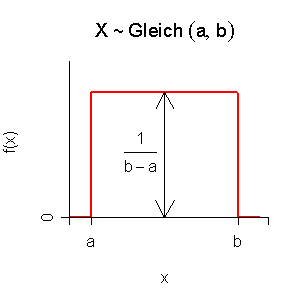
\includegraphics[width=0.42\textwidth]{img/gleichverteilung1}
    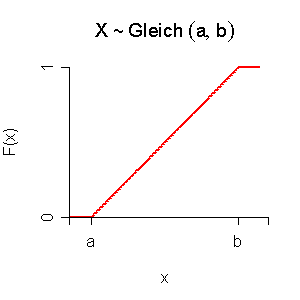
\includegraphics[width=0.42\textwidth]{img/gleichverteilung2}
      \caption{Quelle: Wikipedia}
\end{figure}
 \end{frame}




\begin{frame}
    \frametitle{Verteilungen}
\framesubtitle{}

\begin{block}{Gleichverteilung}
Sei $X \sim $U(a,b).
\begin{align*}
& \mathbb{E}(X) =\int\limits_{-\infty}^\infty x \cdot f(x)\,dx = \frac 1{b-a}\int\limits_a^b x\cdot 1\,dx = \frac 12\frac{b^2-a^2}{b-a} = \frac{a+b}2 \\
& \mathbb{V}(X) = \operatorname{E}(X^2) - \left({\operatorname{E}(X)} \right)^2  = \frac{1}{b - a}\int\limits_a^b {x^2 \cdot 1\,dx}  - \left( {\frac{a + b}{2}} \right)^2  \\
 & = \frac{1}{3}\frac{b^3  - a^3}{b - a} - \left( {\frac{a + b}{2}} \right)^2 \\
    &= \frac{1}{12}\left( {4b^2  + 4ab + 4a^2  - 3a^2  - 6ab - 3b^2 } \right) = \frac{1}{12}(b - a)^2
\end{align*}
\end{block}
 \end{frame}



\begin{frame}
    \frametitle{Verteilungen}
\framesubtitle{}

\begin{block}{Normalverteilung}
Die Normalverteilung $N{(\mu,\sigma^2)}$ auf $\mathbb{R}$ ist definiert durch
\begin{align*}
& \text{Dichte: } f (x) : = \frac 1{\sigma \sqrt{2\pi}}e^{- \frac {1}{2} (\frac{x- \mu}{ \sigma})^2} \\
&  \Rightarrow \text{Verteilung: } F(x) = N{(\mu,\sigma^2)}(-\infty , x) =  \int_{-\infty}^{x}  \frac 1{\sigma \sqrt{2\pi}}e^{- \frac {1}{2} (\frac{t- \mu}{ \sigma})^2}dt\\
\end{align*}

\end{block}
 \end{frame}



\begin{frame}
    \frametitle{ Verteilungen}
\framesubtitle{}
\begin{figure}[htp]
      \centering
    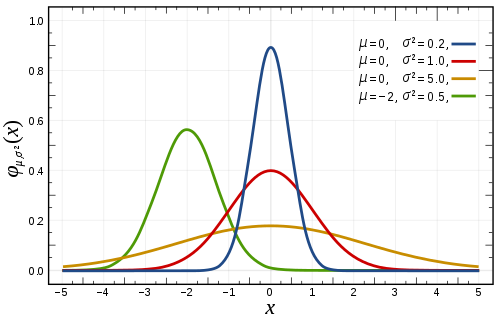
\includegraphics[width=0.45\textwidth]{img/normal}
    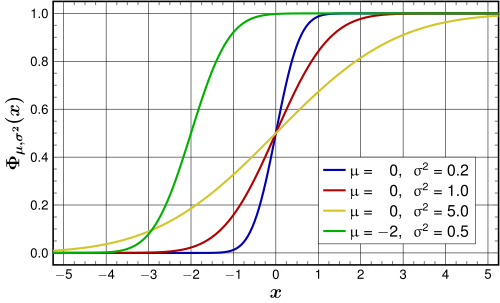
\includegraphics[width=0.45\textwidth]{img/normaldist}
      \caption{Quelle: Wikipedia}
\end{figure}

 \end{frame}


\begin{frame}
    \frametitle{Verteilungen}
\framesubtitle{}

\begin{block}{Normalverteilung}
Sei $X \sim N(\mu, \sigma^2)$.
\begin{align*}
& \mathbb{E}(X) = \mu \\
& \mathbb{V}(X) = \sigma^2
\end{align*}
\end{block}
 \end{frame}



\begin{frame}
    \frametitle{ Verteilungen}
\framesubtitle{}

\begin{block}{Poissonverteilung}
Die Poissonverteilung  $Pois (\lambda)$ auf $\mathbb{N}_{\geq 0}$ ist definiert durch
\begin{align*}
& P_\lambda (k) = \frac{\lambda^k}{k!}\, \mathrm{e}^{-\lambda} \\
& \Rightarrow F_{\lambda}(n)=\sum_{k=0}^n P_\lambda (k) = \mathrm{e}^{-\lambda} \sum_{k=0}^n \frac{\lambda^k}{k!}
\end{align*}
\end{block}
\begin{figure}[htp]
      \centering
    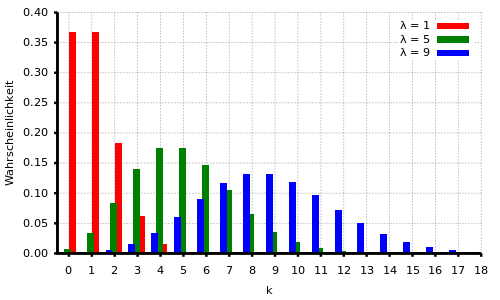
\includegraphics[width=0.55\textwidth]{img/Poisson}
      \caption{Quelle: Wikipedia}
\end{figure}
 \end{frame}



\begin{frame}
    \frametitle{ Verteilungen}
\framesubtitle{}

\begin{block}{Poisson Verteilung}
Die Poisson Verteilung beschreibt das Auftreten von seltenen Ereignissen und spielt bei Zählprozessen eine wichtige Rolle.
\end{block}
\begin{block}{Poisson Verteilung}
$X\sim Pois (\lambda)$ 
\begin{align*}
& \mathbb{E}(X) = \lambda \\
& \mathbb{V}(X) = \lambda
\end{align*}
\end{block}
 \end{frame}


\begin{frame}
    \frametitle{Verteilungen}
\framesubtitle{}

\begin{block}{Bernoulliverteilung}
Die Bernoulliverteilung  Für $\Omega = \{ 0, 1\}$ und $p \in [0,1]$ ist definiert durch
\begin{align*}
P (\omega) = p^{\omega} (1-p)^{1 -\omega}
\end{align*}
\end{block}

\begin{block}{Beispiele}

\begin{itemize}
\item Werfen einer Münze: Kopf (Erfolg), $p=1/2$, und Zahl (Misserfolg), $q=1/2$.
\item Werfen eines Würfels, wobei nur eine 6 als Erfolg gewertet wird: $p=1/6, q=5/6$.
\item Qualitätsprüfung (einwandfrei, nicht einwandfrei).
\item Betrachte sehr kleines Raum/Zeit-Intervall: Ereignis tritt ein $(p \gtrapprox 0)$, tritt nicht ein $(q\lessapprox 1)$.
\end{itemize}

\end{block}
 \end{frame}




\begin{frame}
    \frametitle{ Verteilungen}
\framesubtitle{}

\begin{block}{Binomialverteilung}
$B(k,  p,n)= \binom nk p^k (1-p)^{n-k} $
\end{block}
\begin{block}{Binomialverteilung}
$X_1, \cdots ,X_n \sim B \Rightarrow \sum X_i  \sim B$
\end{block}

\begin{figure}[htp]
      \centering
    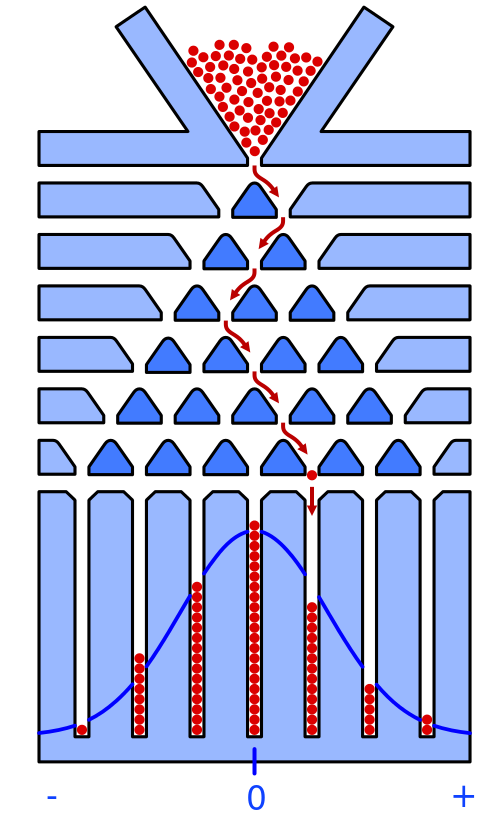
\includegraphics[width=0.25\textwidth]{img/Galton}
      \caption{Quelle: Wikipedia}
\end{figure}
 \end{frame}


\begin{frame}
    \frametitle{Erwartungswert}
\framesubtitle{}
\begin{block}{Markov Ungleichung}
Sei $Y : \Omega \to \mathbb{R}$  eine  reelle, integrierbare  Zufallsvariable und $f : [0, \infty) \to [0, \infty)$ monoton wachsend.
Dann gilt für alle $\epsilon > 0$ mit $f(\epsilon) > 0$
\begin{align*}
P (|Y |  \geq \epsilon) \leq \frac{\mathbb{E} (f \circ |Y|)}{f(\epsilon)}
\end{align*}
\end{block}

 \end{frame}


 \begin{frame}
    \frametitle{Erwartungswert}
\framesubtitle{}

\begin{block}{Beweis}
    Für $f(x)=x$ und $ X > 0$
\begin{itemize}
   
  \item Zerlegung in zwei Teile:
    \[
      X = X \,\mathbf{1}_{\{X<a\}} \;+\; X \,\mathbf{1}_{\{X\ge a\}},
    \]
    wobei $\mathbf{1}_{\{\cdot\}}$ die Indikatorfunktion ist.
  \item Beachte, dass
    \[
      X\,\mathbf{1}_{\{X<a\}} < a,
      \qquad
      X\,\mathbf{1}_{\{X\ge a\}} \;\ge\; a\,\mathbf{1}_{\{X\ge a\}}.
    \]
  \item Daher
    \[
      \begin{aligned}
        \mathbb{E}[X]
        &= \mathbb{E}\bigl[X\,\mathbf{1}_{\{X<a\}}\bigr]
         + \mathbb{E}\bigl[X\,\mathbf{1}_{\{X\ge a\}}\bigr] \\
        &\ge 0 \;+\; a\,\mathbb{E}\bigl[\mathbf{1}_{\{X\ge a\}}\bigr]
         = a\,\Pr(X \ge a).
      \end{aligned}
    \]
  \item Daraus folgt unmittelbar die \emph{Markov‐Ungleichung}:
      $\Pr(X \ge a) \;\le\; \frac{\mathbb{E}[X]}{a}$.
\end{itemize}
\end{block}
 \end{frame}


 \begin{frame}
    \frametitle{Erwartungswert}
\framesubtitle{}

\begin{block}{Beweis}
Da $f(\epsilon) 1_{\{ |Y| \geq  \epsilon \} } \leq f \circ |Y|$ folgt
\begin{align*}
f(\epsilon) P(|Y| \geq \epsilon) = & f(\epsilon) \mathbb{E}(1_{\{ |Y| \geq  \epsilon \} }) = \mathbb{E}( f(\epsilon) 1_{\{ |Y| \geq  \epsilon \} }) \\
\leq & \mathbb{E}( f \circ |Y|)
\end{align*}
\end{block}
 \end{frame}

\begin{frame}
    \frametitle{Erwartungswert}
\framesubtitle{}
\begin{block}{Tschebyscheff-Ungleichung}
Für eine reelle, integrierbare und quadratintegrierbare  Zufallsvariable $Y : \Omega \to \mathbb{R}$  gilt:
\begin{align*}
P (|Y  - \mathbb{E} (Y)|  \geq \epsilon) \leq \frac{\mathbb{V} (Y)}{ \epsilon^2} 
\end{align*}
\end{block}
\begin{block}{Beweis}
Folgt direkt aus der Markov-Ungleichung mit $Y' = Y -\mathbb{E}(Y)$ und $f(x) = x^2$
\end{block}
 \end{frame}


\begin{frame}
    \frametitle{Highlight}
\framesubtitle{}
\begin{figure}[htp]
      \centering
    
\includegraphics[width=0.9\textwidth]{img/firework}
\end{figure}
 \end{frame}


\begin{frame}
    \frametitle{Erwartungswert}
\framesubtitle{}
\begin{block}{Schwaches Gesetz der großen Zahlen}
Seien $X_i : \Omega \to \mathbb{R}$ unabhängige, reelle Zufallsvariablen (uiv, iid(englisch)) mit $\mathbb{E}(X_i) = \mu < \infty$ und $\mathbb{V}(X_i) = \sigma < \infty$, dann gilt
\begin{align*}
P \bigl ( \bigl | \frac{1}{n} \sum_{i=1}^{n} X_i - \mu \bigr |  \geq \epsilon \bigr ) \leq \frac{\sigma}{ n \cdot \epsilon^2} \; \; \underset{n \to \infty}{\longrightarrow} 0
\end{align*}
(stochastische Konvergenz). 
\end{block}
 \end{frame}


\begin{frame}
    \frametitle{Erwartungswert}
\framesubtitle{}
\begin{block}{Beweis}
Mit $Y_n =  \frac{1}{n} \sum_{i=1}^{n}  X_i - \mu$ ist $\mathbb{E}(Y_n) =  \frac{1}{n} \sum_{i=1}^{n} \mathbb{E}( X_i - \mu) = 0$ und 
$\mathbb{V}(Y_n) =  \frac{1}{n^2} \sum_{i=1}^{n} \mathbb{V}( X_i ) = \frac{\sigma}{n}$. Aus der Tschebyscheff-Ungleichung folgt die Behauptung.
\end{block}
 \end{frame}


\begin{frame}
    \frametitle{Erwartungswert}
\framesubtitle{}

\begin{figure}[htp]
      \centering
    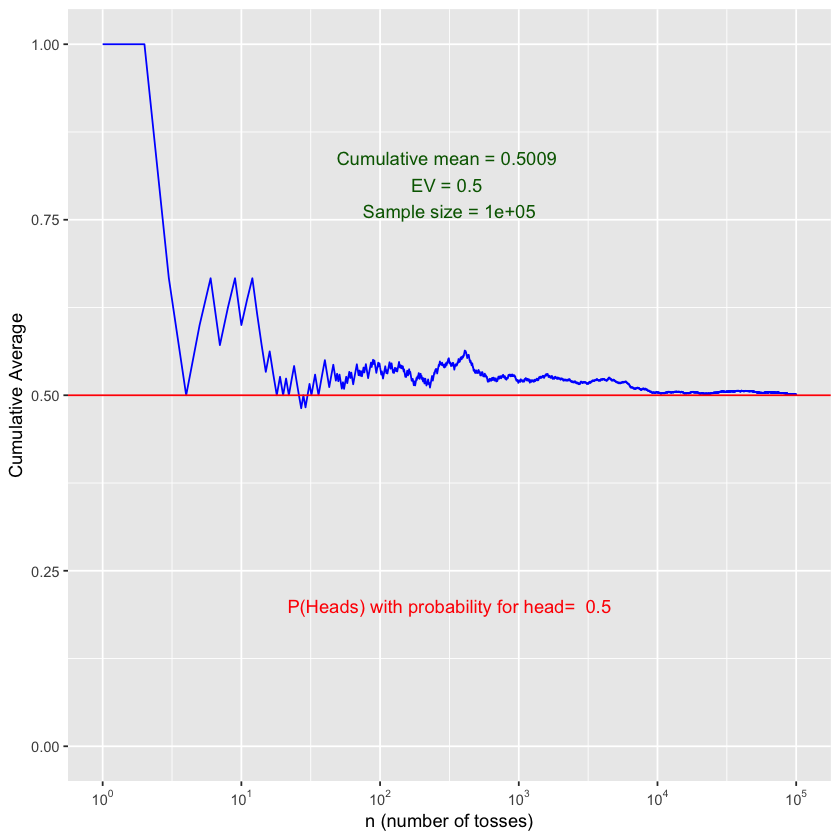
\includegraphics[width=0.86\textwidth]{img/sgdz}
      \caption{Quelle: Wikipedia}
\end{figure}
 \end{frame}



 
\end{document}

